\def\iangle{-30} % Angle of the inclined plane
\def\down{-90}
\def\arcr{0.5cm} % Radius of the arc used to indicate angles
\def\longueurFil{2.5}

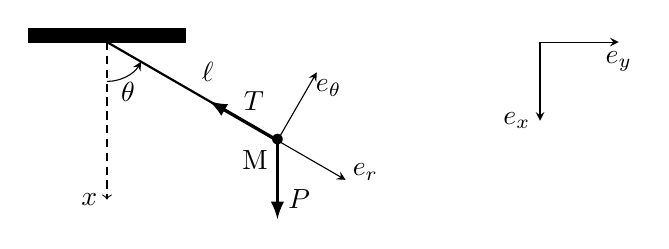
\begin{tikzpicture}[
    force/.style={->,>=latex,draw=\JRLblue,very thick,nodes={\JRLblue}},
    base/.style={>=latex},
    axis/.style={->,>=stealth},
    M/.style={rectangle,draw,fill=lightgray,minimum size=0.5cm,thin},
    m/.style={rectangle,draw=black,fill=lightgray,minimum size=0.3cm,thin},
    plane/.style={draw=\JRLblueC,fill=\JRLblueC},	
	]

    \draw [plane] (-1,0) rectangle (1,5pt) ;%node [midway, above] {$O$};
    \draw[\JRLblueF] (-1,0)--++(2,0);
	
    \draw [densely dashed,->] (0,0) -- (0,-2) node [left] {$x$};
    \draw[thick] (0,0) coordinate (base) -- coordinate[pos=0.5] (mid)++(\iangle:\longueurFil) coordinate (M);
    \draw [axis] (M) -- ++(\iangle:1) node [xshift = 2.5mm, yshift = 1mm] {$\vv{e_r}$};
    \draw [axis] (M) -- ++(\iangle+90:1) node [xshift = 1.5mm, yshift = -2mm] {$\vv{e_\theta}$};
    \draw (mid) node [above right] {$\ell$};
    
    \draw[->,>=stealth] (base)++(0,-\arcr) arc (-90:\iangle:\arcr);
    \path (base)++(\iangle-15:\arcr+5pt) node[left, yshift = -1.5mm] {$\theta$};
    
    \draw[force] (M) -- ++(0,-1) node [above right] {$\vv{P}$};
    \draw[force] (M) -- ++(180+\iangle:1) node [right, xshift=3mm] {$\vv{T}$};
    \draw (M)node {$\bullet$} node [below left] {M};
    
    \coordinate (O) at (5.5, 0) {};
    \draw [->,axis] (O) -- ++(1,0) node [below] {$\vv{e_y}$};
    \draw [->,axis] (O) --++ (0,-1) node [left] {$\vv{e_x}$};
\end{tikzpicture}
